\RequirePackage{luatex85}
\documentclass[9pt,aspectratio=169]{beamer}

\usepackage{luamplib}
  \mplibsetformat{metafun}
  \mplibtextextlabel{enable}
\everymplib{input mpcolornames; input repere; input macros; input featpost3Dplus2D; beginfig(1);}
\everyendmplib{endfig;}

\usetheme{graham}

\title{Kvantik problems,\\ September 2022}
% \subtitle[Graham Middle School]{Graham Middle School Math Olympiad Team}

\begin{document}
\maketitle

\begin{frame}{Problem 1 \hspace*{5cm} Problem 2}
  \begin{columns}[T]
    \begin{column}{0.5\textwidth}
      \begin{problem}
        During a tea party, everybody was treated with candies. Peter and Basil take two pieces of candy of each type but eat only $10$ pieces of candy each; the rest they take home. How many types of candy were at the tea party if Peter took home only three types of candy and Basil took home six types of candy?
      \end{problem}

      Peter can't take home more than $3 \times 2 = 6$ candies and Basil can't take home less than $6$ candies. Since kids take home the same amount of candies, both of them have to take home $6$ candies. So each of them receives $16$ candies and the total number of candies is $16/2 = \boxed{8}$.
    \end{column}
    \begin{column}{0.5\textwidth}
      \begin{problem}
        Lillebror and Karlsson-on-the-Roof share a $5\times 6$ cake decorated with cherries (see picture). Can Karlsson cut the cake into two congruent (with the same shape and size) parts so that he can get all the cherries?
      \end{problem}

      Karlsson can get cut the cake like this:
      \begin{center}
        \leavevmode
        \begin{mplibcode}
          u := 0.5cm;
          for i := 0 upto 6:
            draw (i*u, 0u)--(i*u, 5u) withcolor 0.7white;
          endfor;
          for i := 0 upto 5:
            draw (0u, i*u)--(6u, i*u) withcolor 0.7white;
          endfor;
          draw (0.5u, 2.5u) withpen pencircle scaled 0.5u withcolor red;
          draw (2.5u, 2.5u) withpen pencircle scaled 0.5u withcolor red;
          draw (3.5u, 0.5u) withpen pencircle scaled 0.5u withcolor red;
          draw (3.5u, 3.5u) withpen pencircle scaled 0.5u withcolor red;
          draw (4u, 0u)--(4u, 1u)--(2u, 1u)--(2u, 2u)--(3u, 2u)--(3u, 3u)--(4u, 3u)--(4u, 4u)--(2u, 4u)--(2u, 5u) penextrabold;
        \end{mplibcode}
      \end{center}
    \end{column}
  \end{columns}
\end{frame}

\begin{frame}{Problem 3}
  \begin{columns}[T]
    \begin{column}{0.5\textwidth}
      \begin{problem}
        Harry Potter submerged a stationary ice cube with a side $1$\,cm deep into a tub of water, and all the water, which was closer than $1$\,cm to the cube, had been frozen. Prove that the resulting piece of ice can be cut into several parts and combined into several figures, each of which is a cube, cylinder, or sphere.
      \end{problem}
      \begin{center}
        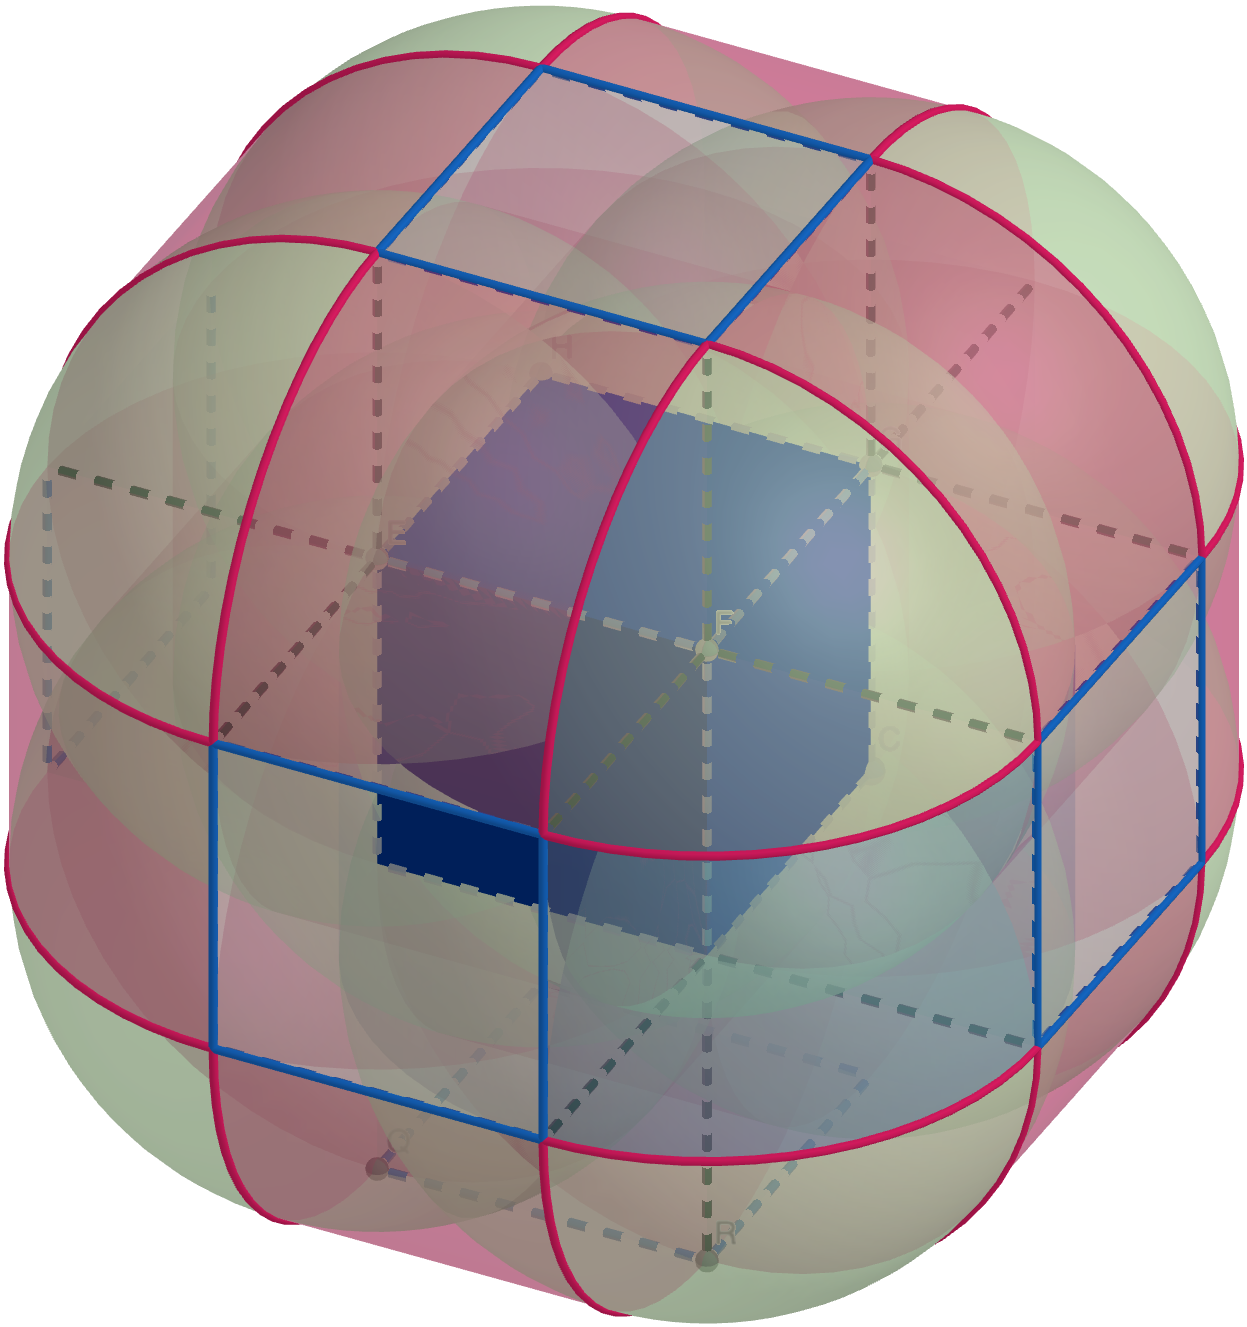
\includegraphics[width=0.6\textwidth]{Kvantik/Harry Potter.png}
      \end{center}
    \end{column}
    \begin{column}{0.5\textwidth}
      Harry Potter will get the piece of ice as shown in the picture. This picture may be cut into $7$ cubes with a side $1$\,cm (one initial cube and $6$ cubes attached to that cube by side, colored blue). $12$ quatres of a cylinder (colored red) may be combined into $3$ cylinders with a radius $1$\,cm and a height $1$\,cm, and remaining $8$ spherical sectors (colored green) can be combined into one sphere with a radius $1$\,cm.
    \end{column}
  \end{columns}
\end{frame}

\begin{frame}{Problem 4}
  \begin{columns}[T]
    \begin{column}{0.5\textwidth}
      \begin{problem}
        On an island, there are $99$ citizens, and everyone is or arguer or yeasayer. Everyone has been asked, in order, who there is more of arguers or yeasayers. Everyone, except the first one, responded this way: a yeasayer responded the same way as the previous islander; the arguer responded contrary to the previous answer. As a result, $75$ islanders responded incorrectly. Is it possible to determine who there are more of arguers or yeasayers?
      \end{problem}
      Every time we asks arguer, the response changed to
      
    \end{column}
    \begin{column}{0.5\textwidth}
      
    \end{column}
  \end{columns}
\end{frame}

\begin{frame}{Problem 5}
  \begin{columns}[T]
    \begin{column}{0.5\textwidth}
      \begin{problem}
        On the cube's vertices, there are $8$ numbers. For any two parallel edges, the sum of numbers is the same. How many of these $8$ numbers can have different values? (Show all options on how many different numbers can be and prove there are no more options.)
      \end{problem}
    \end{column}
    \begin{column}{0.5\textwidth}
      
    \end{column}
  \end{columns}
\end{frame}

\begin{frame}{Problem 40}
  \begin{columns}[T]
    \begin{column}{0.5\textwidth}
      \begin{problem}
        Through a point inside an equilateral triangle, we have drawn three lines parallel to the sides of the triangle. Then we measured the areas of the six pieces we got. Can these areas have exactly three different values?
      \end{problem}
    \end{column}
    \begin{column}{0.5\textwidth}
    \end{column}
  \end{columns}
\end{frame}

% \begin{frame}{Title}
%   \begin{columns}[T]
%     \begin{column}{0.5\textwidth}
%     \end{column}
%     \begin{column}{0.5\textwidth}
%     \end{column}
%   \end{columns}
% \end{frame}

\end{document}
